%Metroplolis Beamer Theme: https://github.com/matze/mtheme
\documentclass[10pt]{beamer}

\setbeamercolor{background canvas}{bg=white}

\usepackage{amsmath}
\usepackage{tikz}
\usepackage{mathdots}
\usepackage{yhmath}
\usepackage{cancel}
\usepackage{color}
\usepackage{siunitx}
\usepackage{array}
\usepackage{multirow}
\usepackage{amssymb}
\usepackage{gensymb}
\usepackage{tabularx}
\usepackage{booktabs}
\usepackage{xcolor}
\usetikzlibrary{fadings}
\usetikzlibrary{patterns}
\usetikzlibrary{shadows.blur}
\usetikzlibrary{shapes}
\usepackage{fontawesome}

\newcommand{\light}[1]{\textcolor{gray}{#1}}

\definecolor{orange}{rgb}{228,108,22}

\usetheme[progressbar=frametitle]{metropolis}
\usepackage{appendixnumberbeamer}

\usepackage{booktabs}
\usepackage[scale=2]{ccicons}

\usepackage{pgfplots}
\usepgfplotslibrary{dateplot}

\usepackage{xspace}
\newcommand{\themename}{\textbf{\textsc{metropolis}}\xspace}

\title{Genetic Circuit Design Automation}
\subtitle{Nielsen et al., \textbf{Science} 2016}
% \date{\today}
\date{}
\author{Gian Hiltbrunner}
\institute{CBB Seminar, ETH Zurich}
\titlegraphic{\vspace{4.5cm}\hfill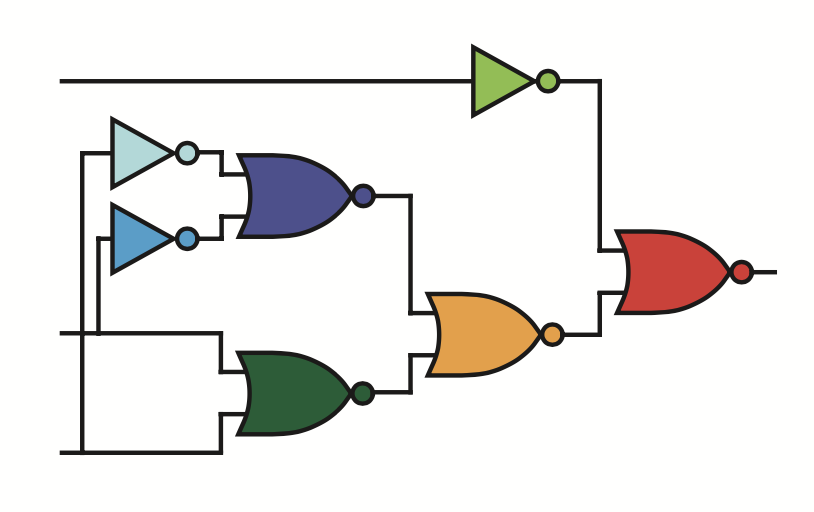
\includegraphics[width = 5cm]{circuit.png}}

\begin{document}

\maketitle

%\begin{frame}{Table of contents}
%  \setbeamertemplate{section in toc}[sections numbered]
%  \tableofcontents%[hideallsubsections]
%\end{frame}

\begin{frame}[fragile]{Introduction}

    {\metroset{block=fill}
      \begin{block}{Situation}
        Biotechnology depends on harnessing the ability of cells to perform computational operations. 
      \end{block}
      \begin{alertblock}{Problem}
        Designing synthetic genetic circuits is time-intensive and unreliable. 
      \end{alertblock}
      \begin{exampleblock}{Proposed Resolution}
        There exist systems used in electrical engineering that describe electronic circuits in special description languages. This system could be adapted for biological applications.
      \end{exampleblock}}
      
\end{frame}

\begin{frame}{Introduction}
  \begin{itemize}[<+- | alert@+>]
    \item Circuits require precise balancing of regulator expression
    \item Many parts are combined to build a circuit, whose functions can vary according to cellular context
    \item Circuits are defined by many states, which can be hard to characterize
    \item Many regulators show toxicity at higher concentrations
    \item[$\rightarrow$] Balancing these issues is difficult, we need computational support
  \end{itemize}
\end{frame}

\begin{frame}[fragile]{Introduction}

    {\metroset{block=fill}
    
      \begin{block}{Situation}
      
        \light{Biotechnology depends on harnessing the ability of cells to perform computational operations. }
      \end{block}
      \begin{block}{Problem}
        \light{Designing synthetic genetic circuits is time-intensive and unreliable.}
      \end{block}
      \begin{exampleblock}{Proposed Resolution}
        There exist systems used in electrical engineering that describe electronic circuits in special description languages. This system could be adapted for biological applications.
      \end{exampleblock}}
      
\end{frame}

\begin{frame}{Technology}

\vspace{0.5cm}
\begin{figure}
    \centering
    \makebox[\textwidth][c]{\includegraphics[width=1\textwidth]{{gate_technology}}}%
\end{figure}

\nocite{Brophy2014PrinciplesDesign} 
\end{frame}

\begin{frame}{Methods}

    \begin{minipage}{.6\textwidth}
        \centering
        \begin{itemize}
            \item Verilog code written by the user describes the logic circuit in textual form. 
            \item Algorithms parse the code and derive a truth table. 
            \item A logic synthesis program uses the truth table to build a corresponding logic circuit. 
            \item The intial NOT/AND design is converted into a NOT/NOR design. 
        \end{itemize}
    \end{minipage}%
    \begin{minipage}{.4\textwidth}
        \centering
        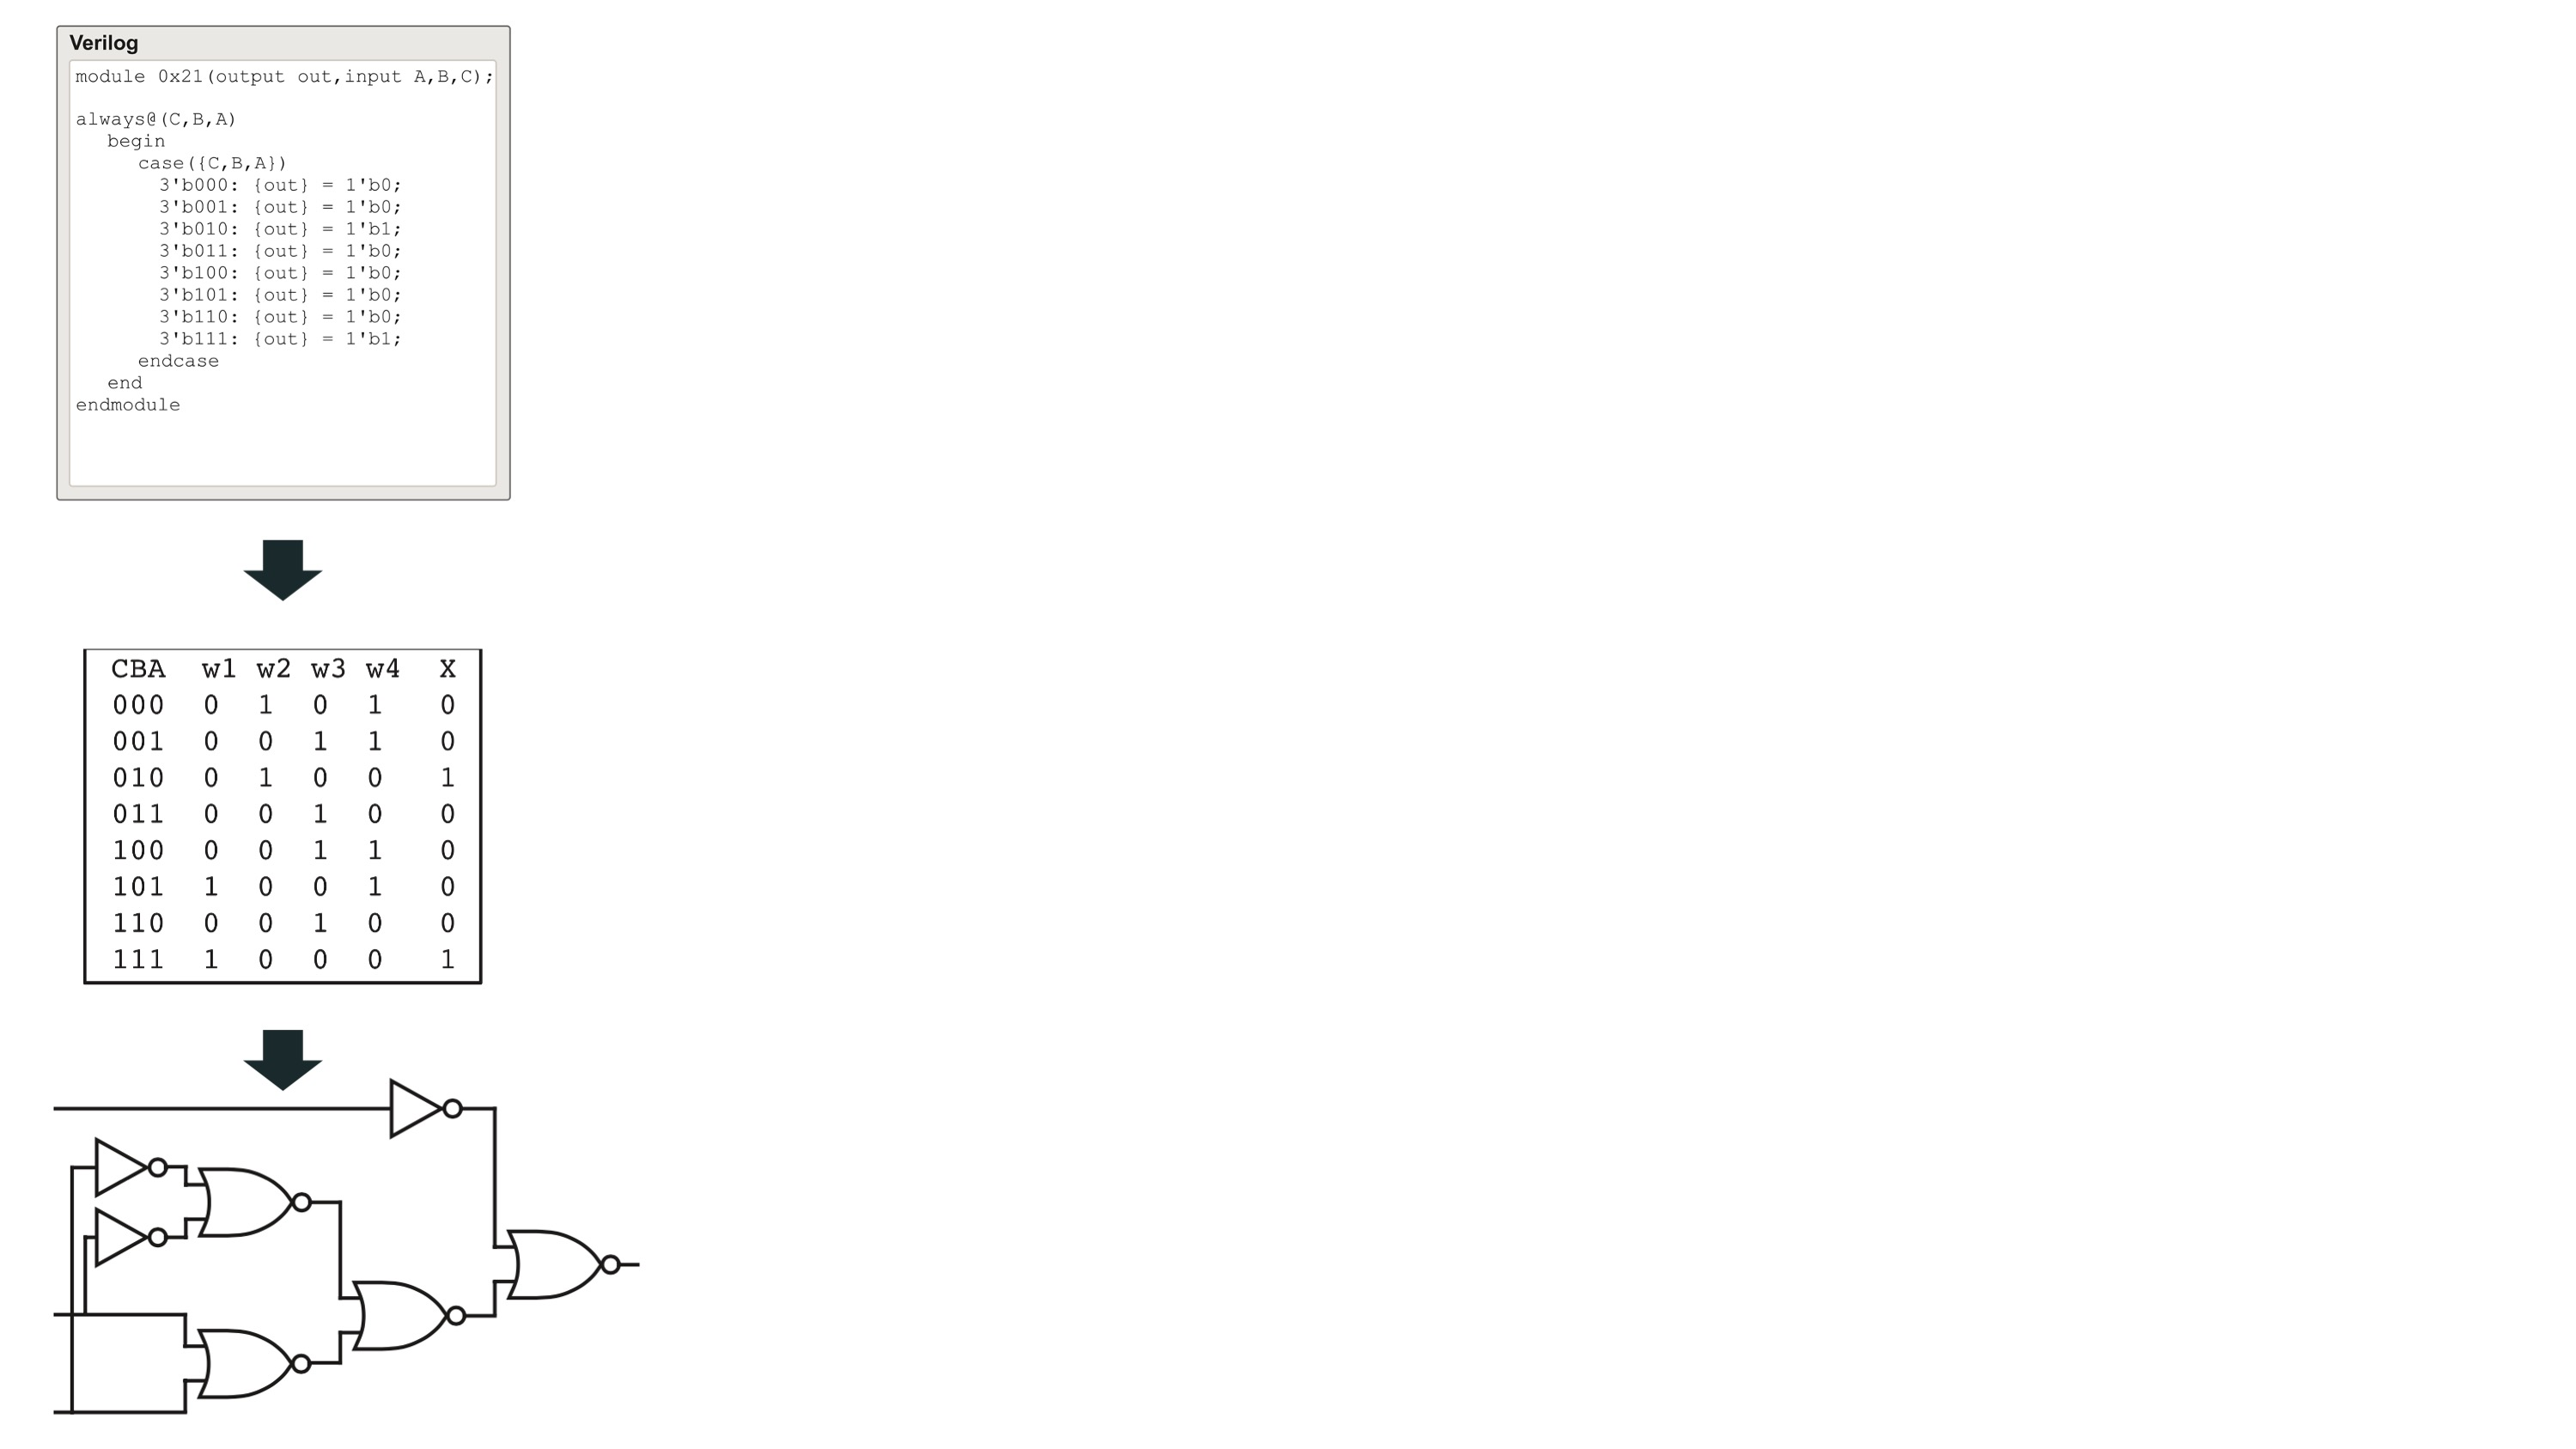
\includegraphics[width=13cm]{overview1.jpg}
    \end{minipage}

\nocite{Nielsen2016GeneticAutomation} 
\end{frame}

\begin{frame}{Methods}
    \begin{minipage}{.4\textwidth}
        \centering
        \begin{itemize}
            \item Circuits are tailor-made for specific organisms and operating conditions. 
            \item Repressors need to be selected appropriately. \item This is done by comparing different variants and selecting the one with the best score: $S = \frac{\text{min}(ON)}{\text{max}(OFF)}$
        \end{itemize}
    \end{minipage}%
    \begin{minipage}{.6\textwidth}
        \centering
        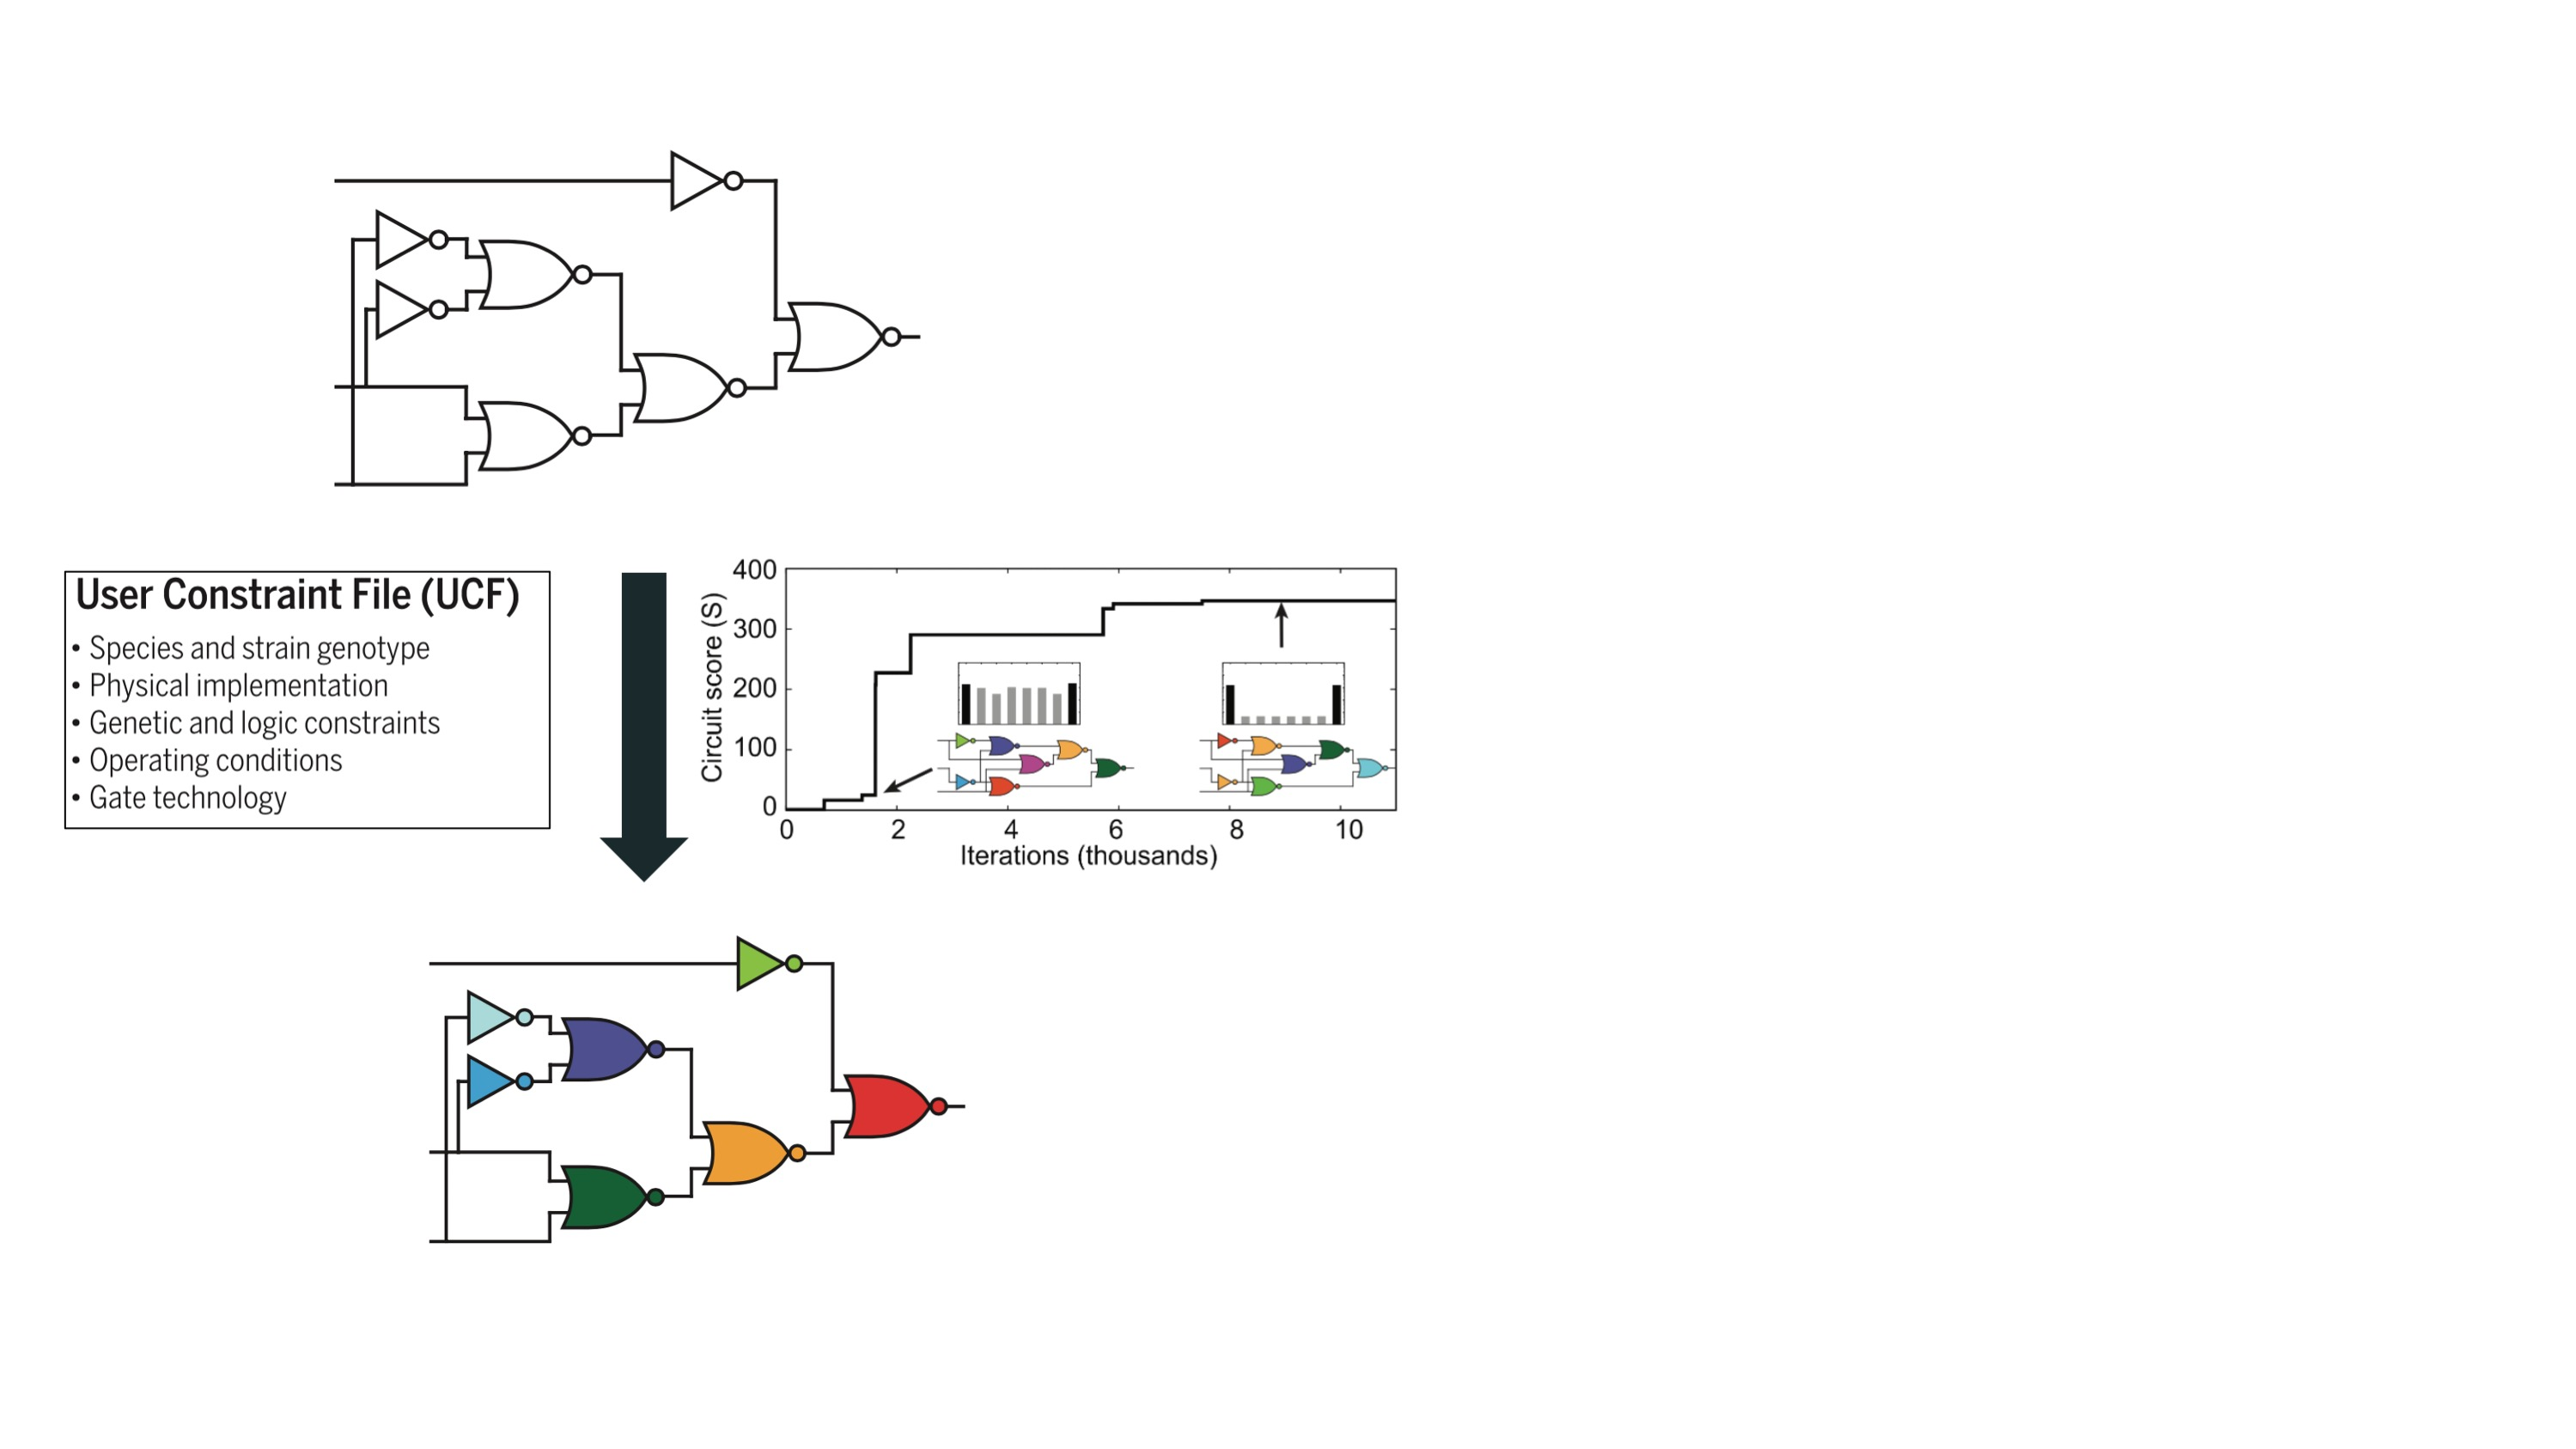
\includegraphics[width=13cm]{overview2.jpg}
    \end{minipage}

\end{frame}


\begin{frame}{Methods}
    \begin{minipage}{.4\textwidth}
        \centering
        \begin{itemize}
            \item The gates are combined into a linear piece of DNA.
            \item The software then simulates the performance of the circuit by simulating the signal propagation trough the gates.  
            \item Finally the software will predict the effect of the gates on cell growth. 
        \end{itemize}
    \end{minipage}%
    \begin{minipage}{.6\textwidth}
        \centering
        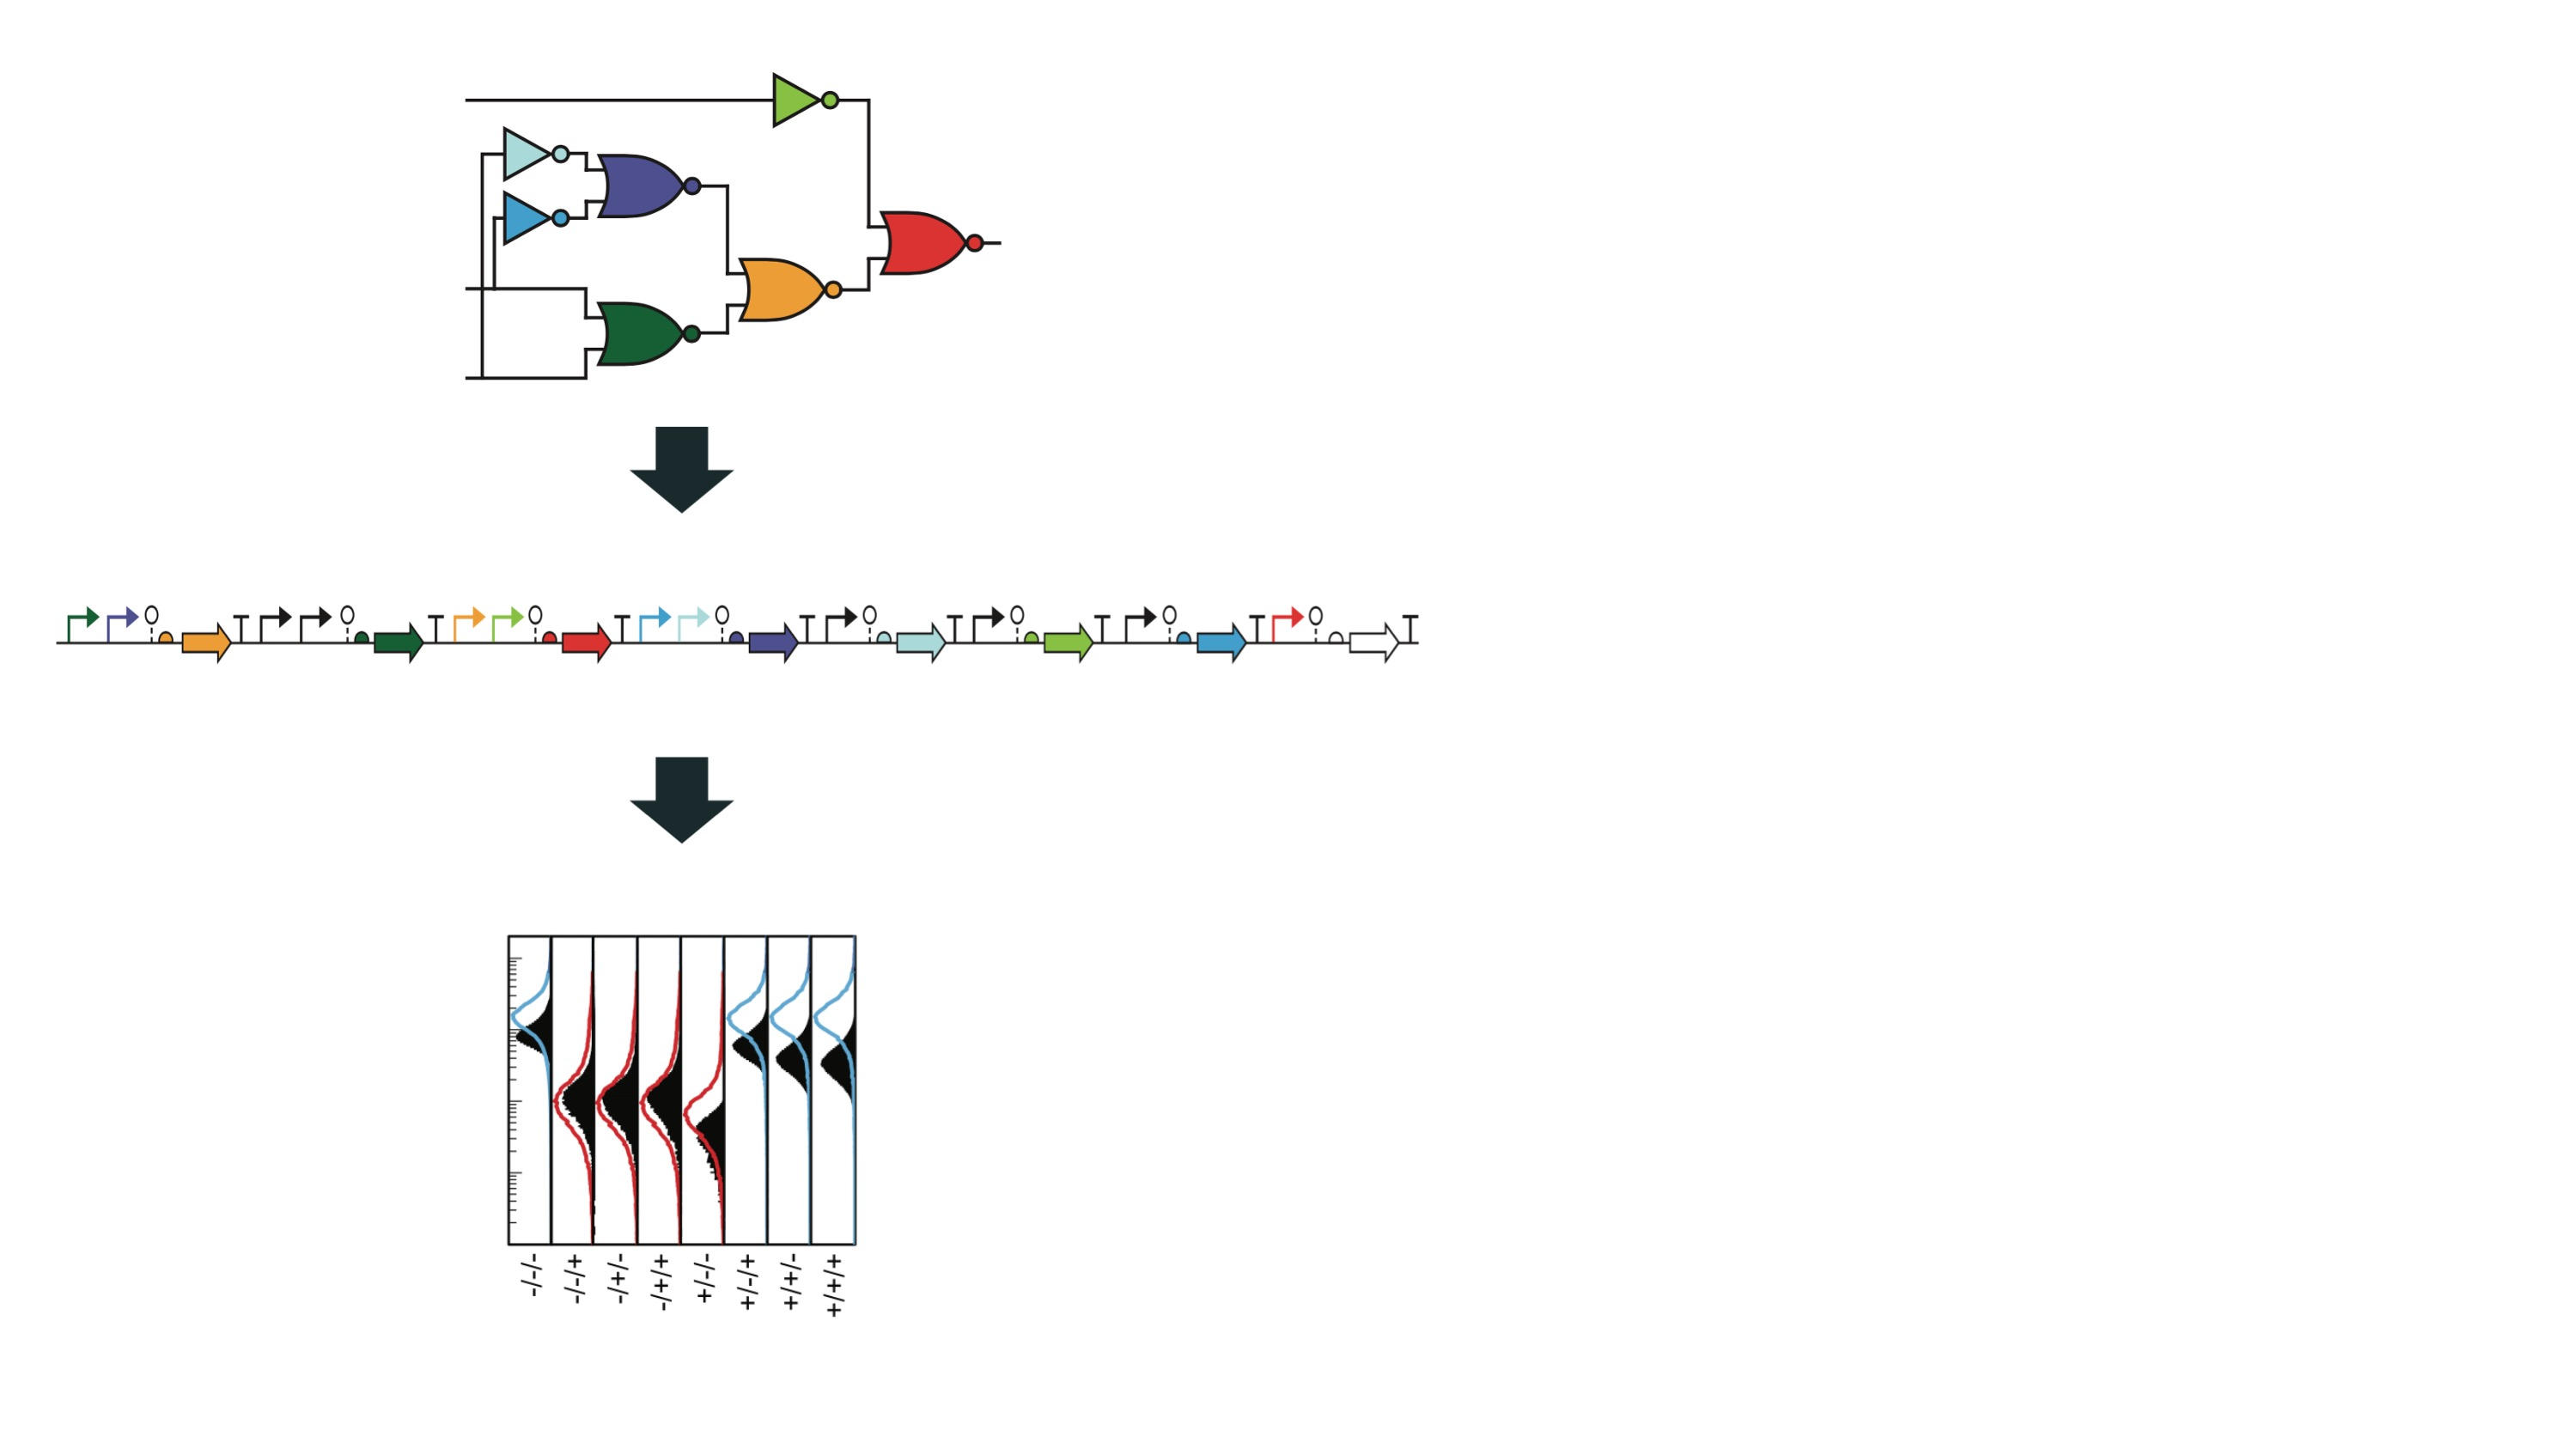
\includegraphics[width=13cm]{overview3.jpg}
    \end{minipage}

\end{frame}

\begin{frame}{Showcase}

    \begin{minipage}{.4\textwidth}
        \centering
        \begin{itemize}
            \item Insulated gates were used to create 52 circuits. 
            \item Circuit output is linked to expression of YFP.
            \item Output states were experimentally measured using flow cytometry and compared to the predictions. 
        \end{itemize}
    \end{minipage}%
    \begin{minipage}{.6\textwidth}
        \centering
        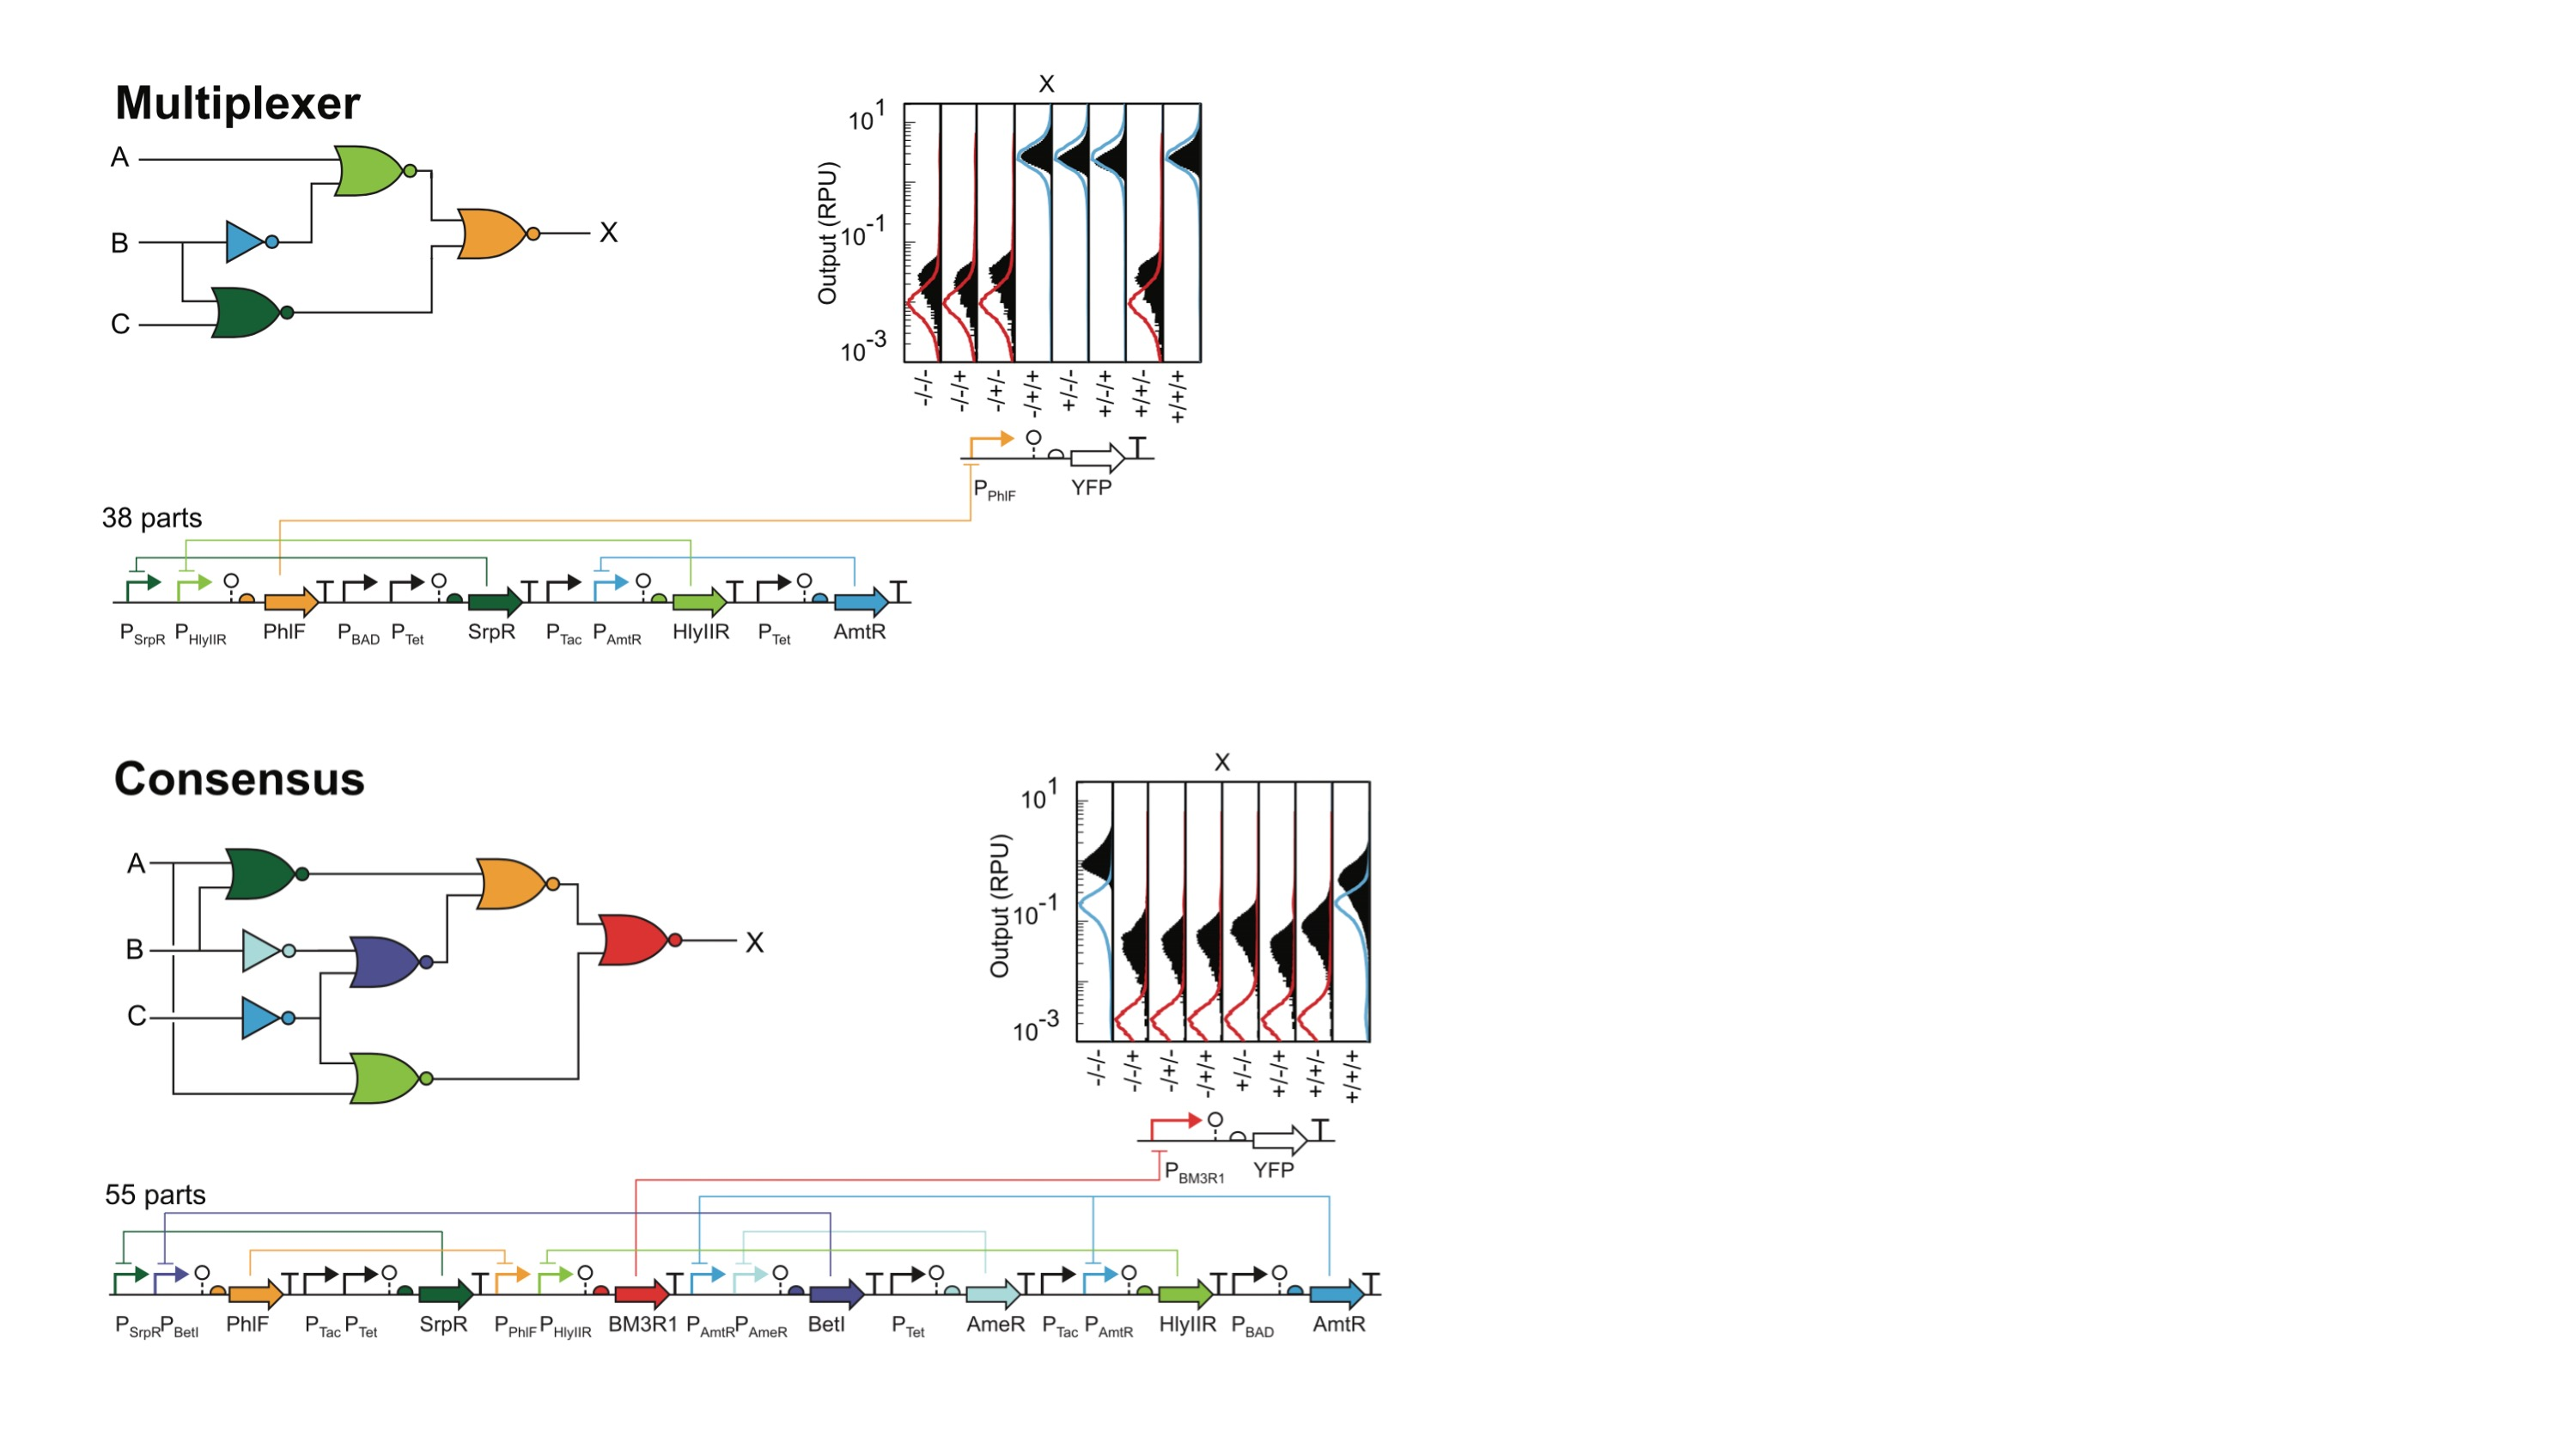
\includegraphics[width=13cm]{examples.jpg}
    \end{minipage}

\end{frame}

\begin{frame}{Challenges}
    \centering
    \begin{minipage}{.4\textwidth}
        \centering
        \begin{itemize}
            \item Often gates can only be functionally connected in one direction.
            \item Some gates significantly influence cell growth.
            \item The probability of finding a functional circuit decreases with increasing number of gates. 
        \end{itemize}
    \end{minipage}%
    \begin{minipage}{.6\textwidth}
        \centering
        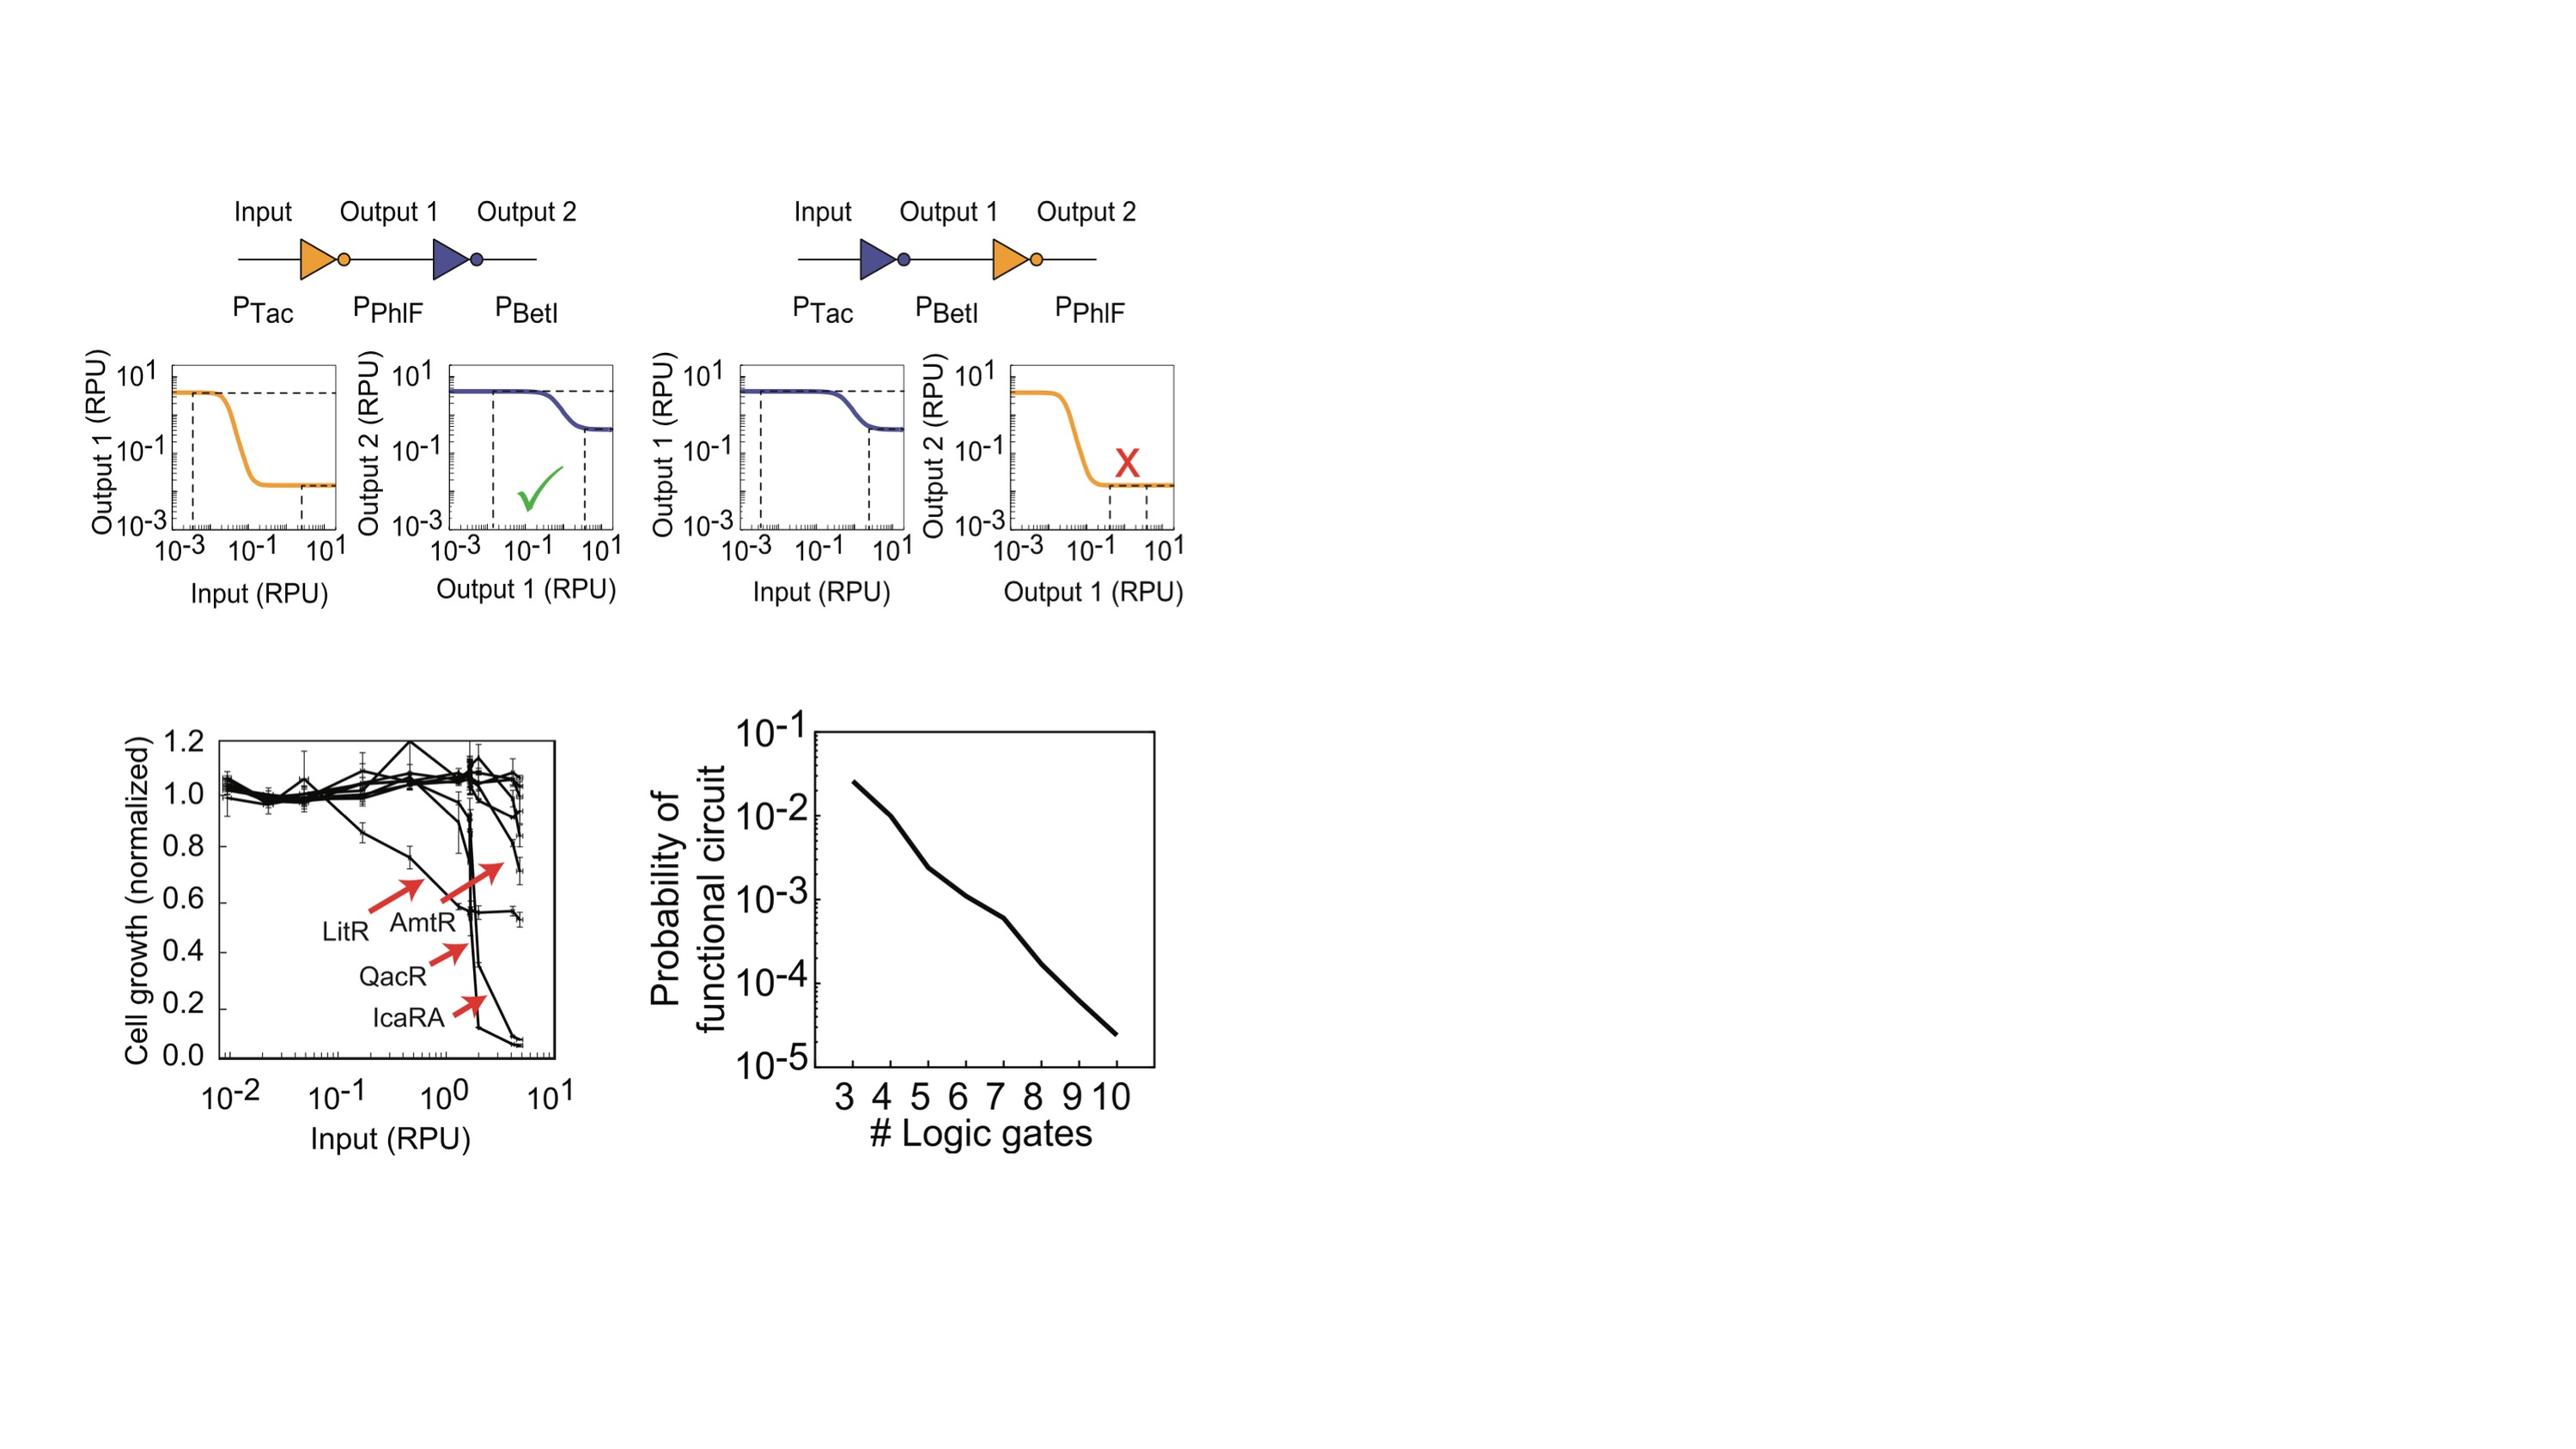
\includegraphics[width=15cm]{challenges.jpg}
    \end{minipage}
\end{frame}

\begin{frame}{Challenges}
    \centering
    \begin{minipage}{.4\textwidth}
        \centering
        \begin{itemize}
            \item There are many unwanted interactions between the gate and the genetic context. 
            \item This occurs due to DNA recombination when gates are too similar and RNA-Polymerase leakage. 
            \item Gates are isolated using strong terminators to block RNA-Polymerase leakage and recombination is hindered
        \end{itemize}
    \end{minipage}%
    \begin{minipage}{.6\textwidth}
        \centering
        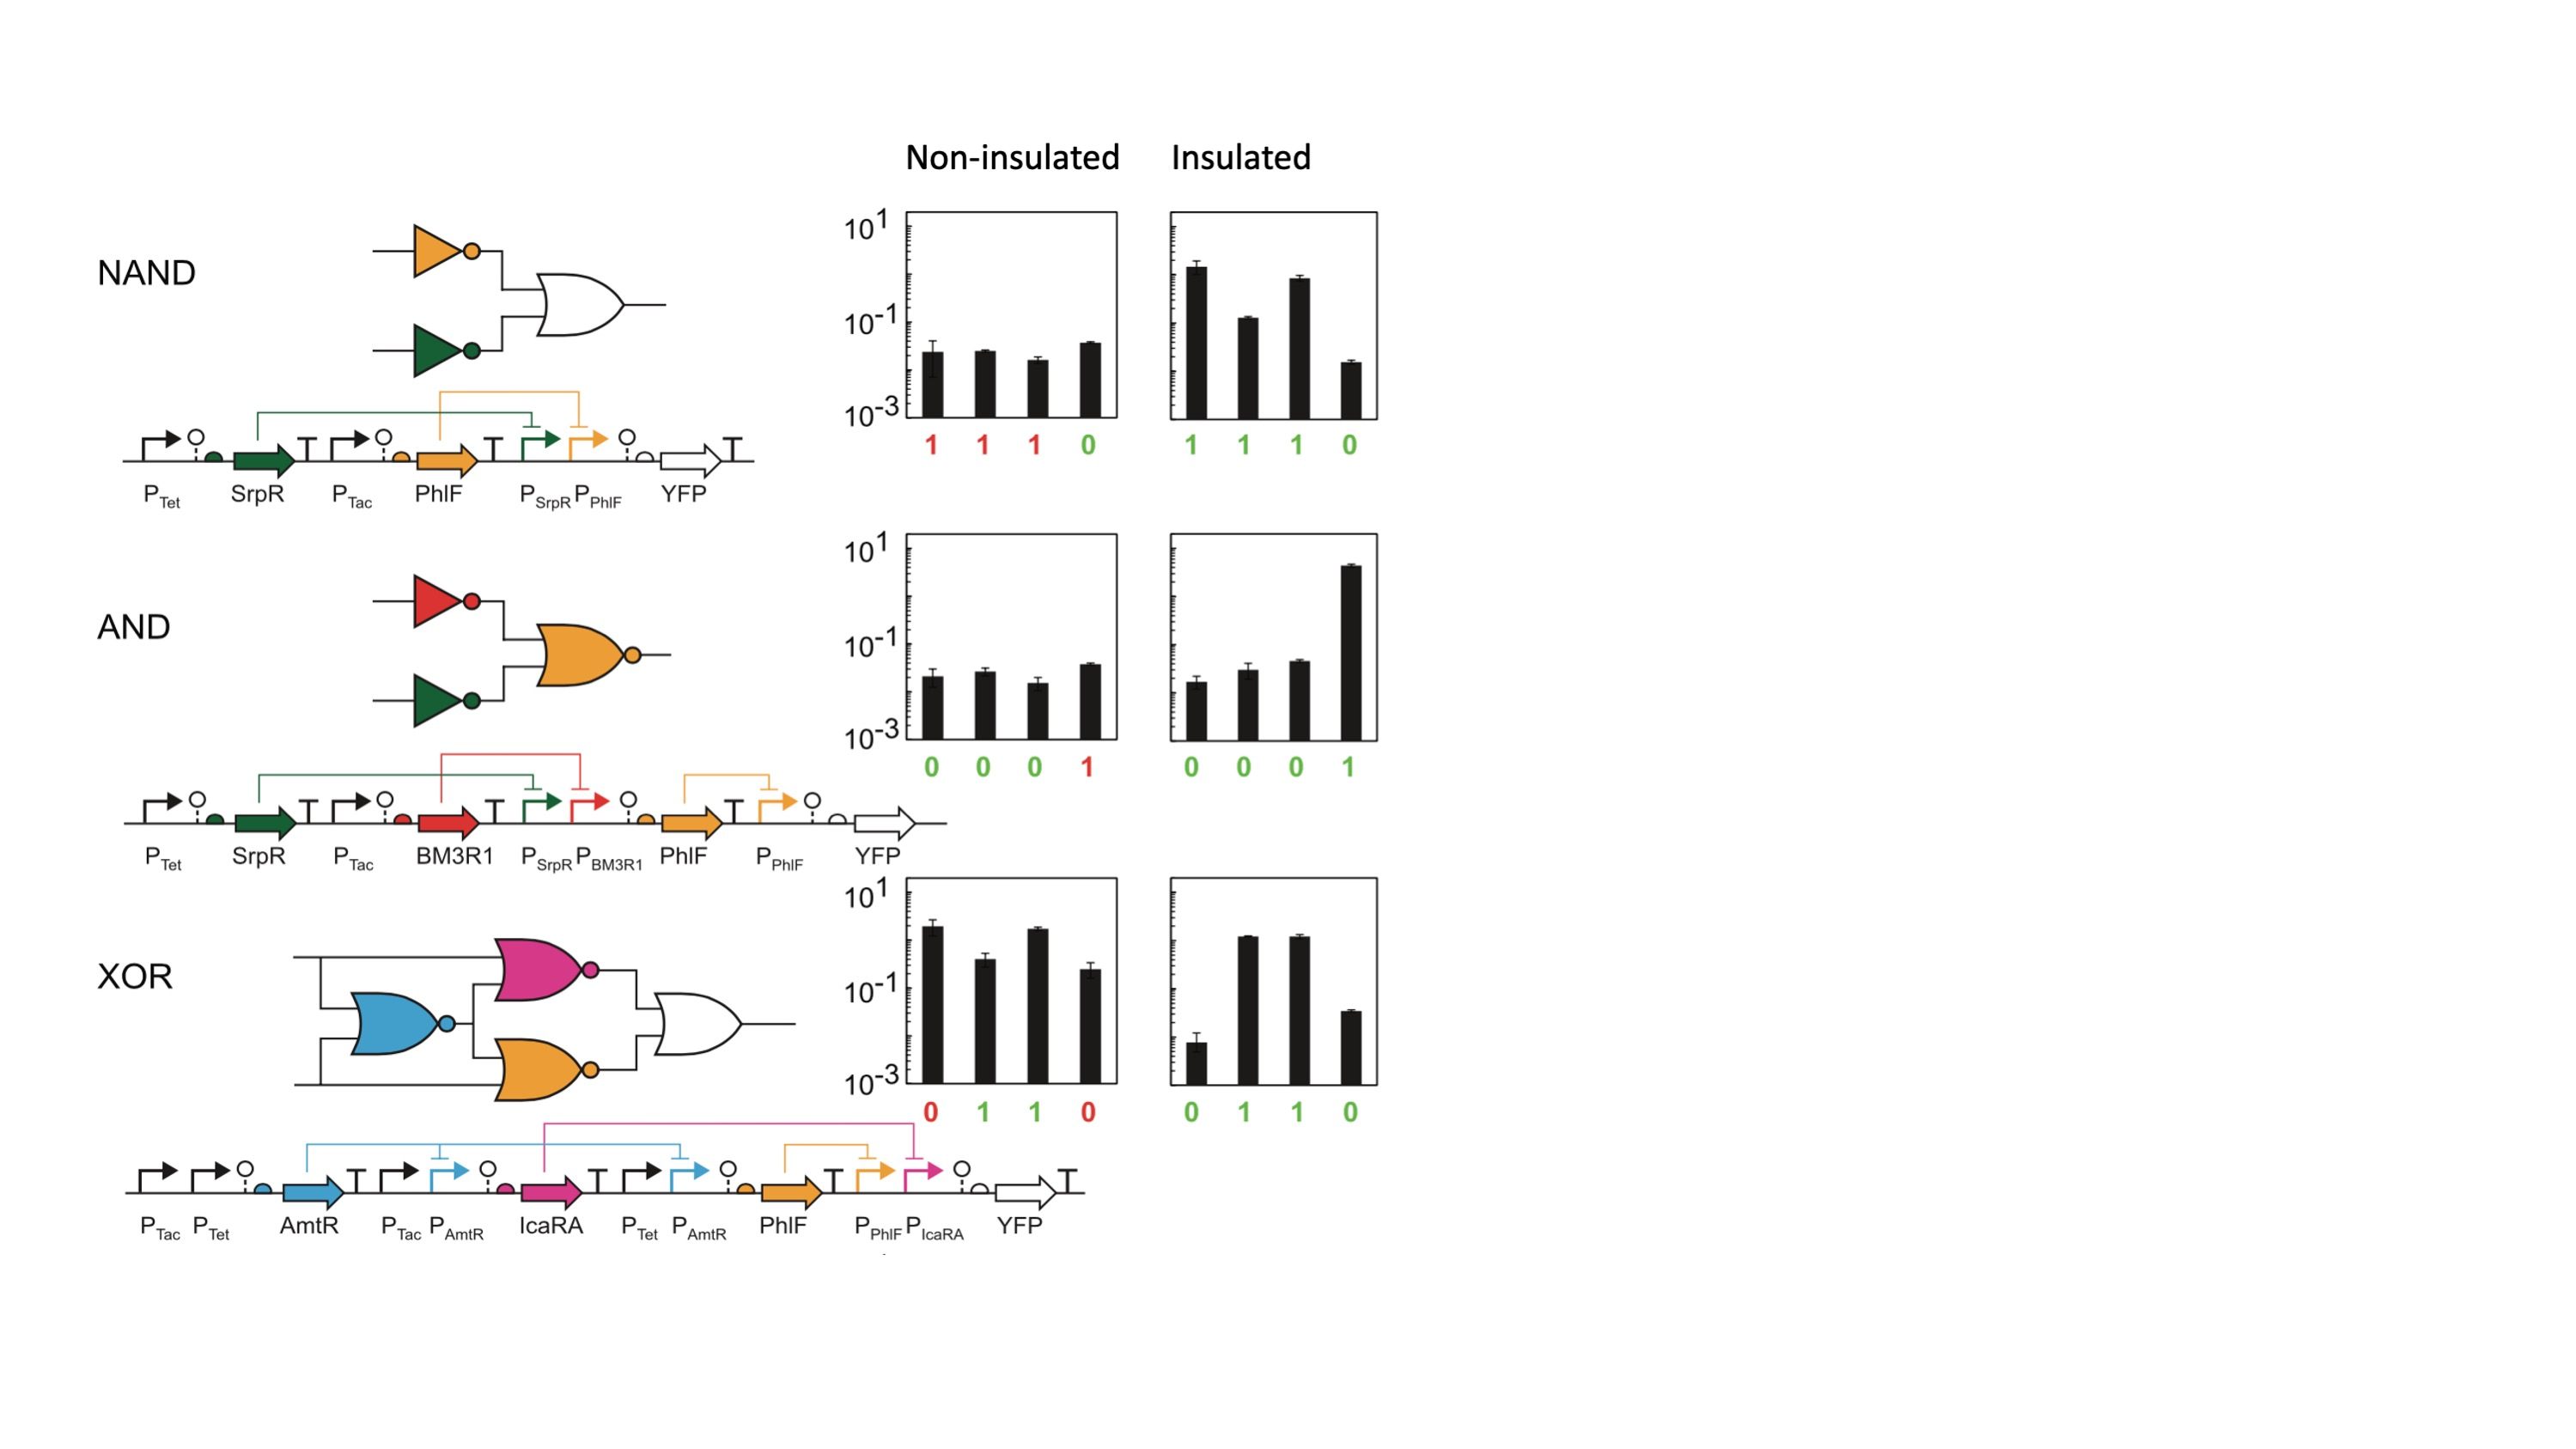
\includegraphics[width=13cm]{challenges_.jpg}
    \end{minipage}
\end{frame}

\begin{frame}{Discussion}
  \begin{itemize}[<+- | alert@+>]
    \item Circuits design has been dominated by manual tinkering, this software automates the selection and concatenation of parts considering additional constraints
    \item This allows for the design of larger more complex multi-part systems
    \item 45 out of 60 designed circuits functioned as expected, the largest containing over 12 promotors, thus doubling previous records 
    \item Of 412 output states 92 \% were found to be correct.
  \end{itemize}
  \nocite{Cloney2016SyntheticDesign}
\end{frame}
    
\begin{frame}{Discussion}
  \begin{itemize}
    \item Circuits design has been dominated by manual tinkering, this software automates the selection and concatenation of parts considering additional constraints
    \item This allows for the design of larger more complex multi-part systems
    \item 45 out of 60 designed circuits functioned as expected, the largest containing over 12 promotors, thus doubling previous records 
    \item Of 412 output states 92 \% were found to be correct.
  \end{itemize}
  \begin{itemize}[<+- | alert@+>]
    \begin{quote}
        \vspace{0.2cm}
        
        "By controlling [...] when genes are turned on to designing therapeutic agents that are programmed to sense a problem in the body and perform a therapeutic action." [R. Cloney]
    \end{quote}
    \end{itemize}
  \nocite{Cloney2016SyntheticDesign}
\end{frame}


{
    \setbeamercolor{palette primary}{fg=black, bg=yellow}
    \begin{frame}[standout]
        \vspace{3cm}
        Questions?
        \vspace{3cm}
        {
            \footnotesize
            \begin{center}{\LARGE \faicon{github}} \url{github.com/gianhiltbrunner/GeneticCircuitDesignAutomationTalk}\end{center}

        } 
    \end{frame}
}

\appendix

\begin{frame}[allowframebreaks]{References}

  \bibliography{references}
  \bibliographystyle{abbrv}

\end{frame}

\begin{frame}{}
    
\end{frame}

\end{document}
